\documentclass[11pt]{article}
\usepackage{geometry}
\geometry{letterpaper}
\geometry{margin=0.5in}


\usepackage[utf8]{inputenc}
\usepackage{listings}
\usepackage{xcolor}
% credit: http://tex.stackexchange.com/questions/68091/how-do-i-add-syntax-coloring-to-my-c-source-code-in-beamer
% https://en.wikibooks.org/wiki/LaTeX/Source_Code_Listings
\lstset{language=C,
        basicstyle=\ttfamily,
        keywordstyle=\color{blue}\ttfamily,
        stringstyle=\color{red}\ttfamily,
        commentstyle=\color{green}\ttfamily,
        morecomment=[l][\color{magenta}]{\#}
}

\title{\textbf{CS 5220 Project 1 Initial Report}}
\author{Stephen McDowell (sjm324)\\ Guantian Zheng (gz94)\\ Jingyang Wang (jw598)}
\date{\textbf{September 2015}}

\usepackage{natbib}
\usepackage{graphicx}
\usepackage{pdfpages}

\newcommand{\tab}{\hspace*{2em}}
\newcommand{\norm}[1]{\lVert#1\rVert}
\newcommand{\sub}{\textsubscript}
\newcommand{\Depth}{2}
\newcommand{\Height}{2}
\newcommand{\Width}{2}

\usepackage{mathtools}
\DeclarePairedDelimiter\ceil{\lceil}{\rceil}
\DeclarePairedDelimiter\floor{\lfloor}{\rfloor}

\usepackage{relsize}
\usepackage{pdfpages}

\def\wl{\par \vspace{\baselineskip}}

\makeatletter
\renewcommand{\maketitle}{\bgroup\setlength{\parindent}{0pt}
\begin{flushleft}
  {\Large \textsc{\@title}}\newline
  \textsc{\@author}
  \rule{\textwidth}{1pt}
\end{flushleft}\egroup
}
\makeatother

\usepackage{fancyhdr}
\pagestyle{fancy}
\rhead{\textsc{Group 018} \thepage}
\renewcommand{\headrulewidth}{0pt}
\setlength{\headheight}{0.5in}

\title{CS 5220: Project 1 Initial Report}
\author{Group 018: Guantian Zheng (gz94), Stephen McDowell (sjm324)}

\begin{document}
\thispagestyle{empty}
\maketitle

\section{Introduction}

Our initial findings for this assignment are somewhat discouraging.  We initially had a bit of trouble figuring out how all of the parts of this assignment fit together.  At this time, we feel that we have a good understanding of how we are supposed to be performing the tasks expected of us, but not much performance has been achieved at this point.

\begin{enumerate}
    \item The first stage of diagnostics was to begin examining how the different permutations of \texttt{i}, \texttt{j}, and \texttt{k} can have an impact on the speed of the basic matrix multiply.

    \item The next natural piece to examine \emph{at a high level} was comparing how \texttt{icc} and \texttt{gcc} compare with one another.  During this phase we used the basic permutations to help us understand which was superior, but have not gone as far as changing the compilation flags -- yet!

    \item We then began examining how these permutations and best-suited compiler can affect the blocked strategy provided in the initial framework, in conjunction with adjusting the \texttt{BLOCK\_SIZE} variable to see its effect on the blocking efficiency.

    \item Where we are currently is trying to query the hardware to programmatically determine the optimal \texttt{BLOCK\_SIZE}, as well as toying with the idea of transposing the \texttt{A} matrix in memory.
\end{enumerate}

\noindent Part of the reason why we have not made as much progress as we would have liked to is because we only have two group members.  This was not really made apparent to us until tonight.

\newpage
\section{Loop Permutations and Compilers}

We experimented with different permutations of the three loop variables \texttt{i}, \texttt{j} and \texttt{k}. Apparently, \texttt{j, k, i} (starting from the outermost loop) gains the most advantage by reading in continuous blocks of matrix \texttt{C} and \texttt{A}. The loops are as follows:

\begin{lstlisting}
    for(j = 0; j < M; ++j) {
        for(k = 0; k < M; ++k) {
            double b_kj = B(k, j);
            for(i = 0; i < M; ++i) {
                C(i, j) += A(i, k) * b_kj;
            }
        }
    }
\end{lstlisting}

\noindent The code for producing these permutations can be found in \texttt{dgemm\_basic-permutations.c}, where you can change \texttt{\#define PERMUTATION} at the top to be 0, 1, 2, 3, 4, or 5 depending on which permutation you want to run.

\noindent When compiling with \texttt{gcc}, we get the following results:

\begin{center}
    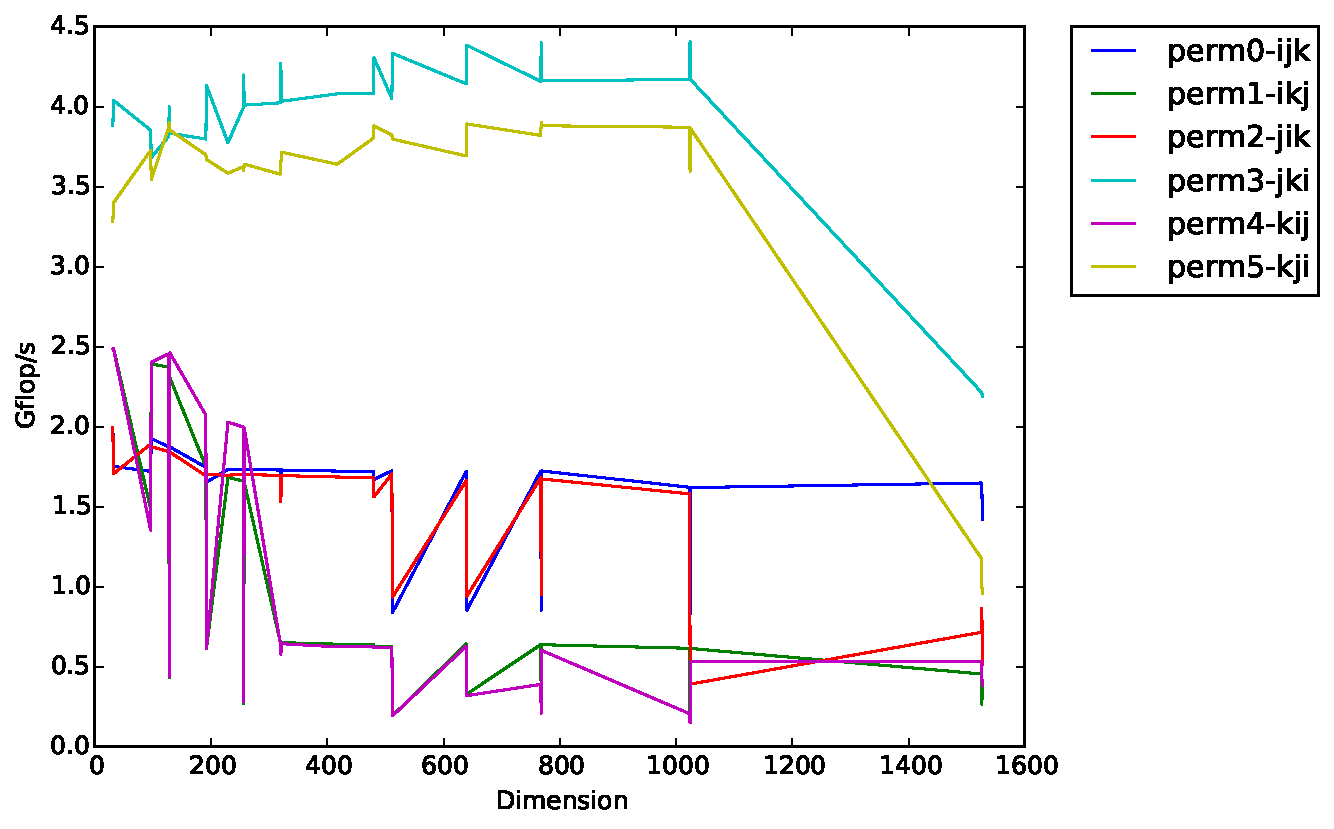
\includegraphics[scale=0.5]{benchmarking/permutations/gcc/timing.pdf}
\end{center}

\noindent noting that the peak is somewhere between 4 and 4.5 Gflop/s.  With the same code being compiled by \texttt{icc}, we get the following trend:

\begin{center}
    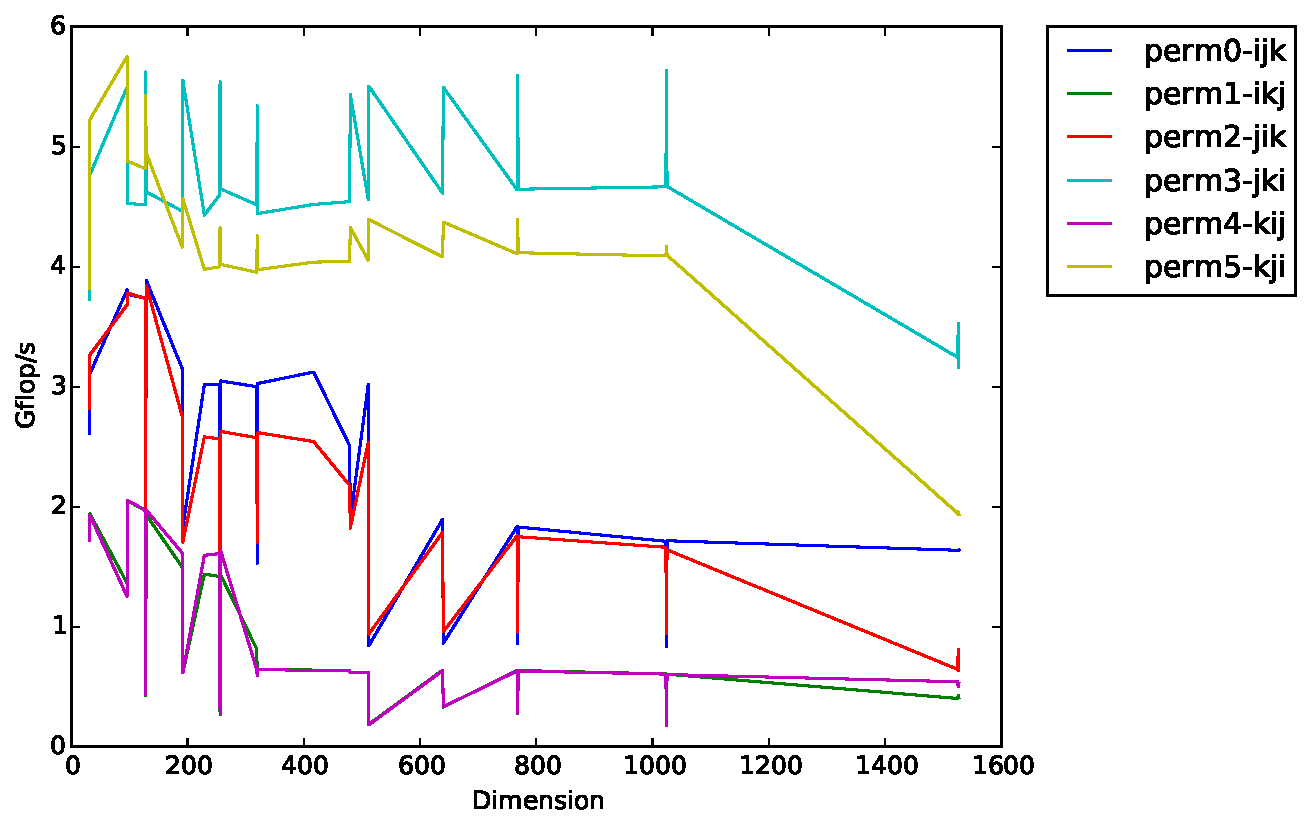
\includegraphics[scale=0.5]{benchmarking/permutations/icc/timing.pdf}
\end{center}

\noindent The difference in performance is not entirely that surprising, given how much of a proponent of \texttt{icc} Prof. Bindel is.  The benchmarks shown above gave a lot of freedom to the compilers, though (the \texttt{Makefile} provided has optimization level 3 for both).  Perhaps a better diagnostic would have been to turn off all optimizations and compare.  But this seems to be a somewhat unrealistic goal, since the point of using the compiler in the first place is that it knows how to speak computer much better than we do.\\

\noindent Lastly, the two plots have been merged in one to demonstrate the superiority of \texttt{icc} when it comes to tuning the basic matrix multiply:

\begin{center}
    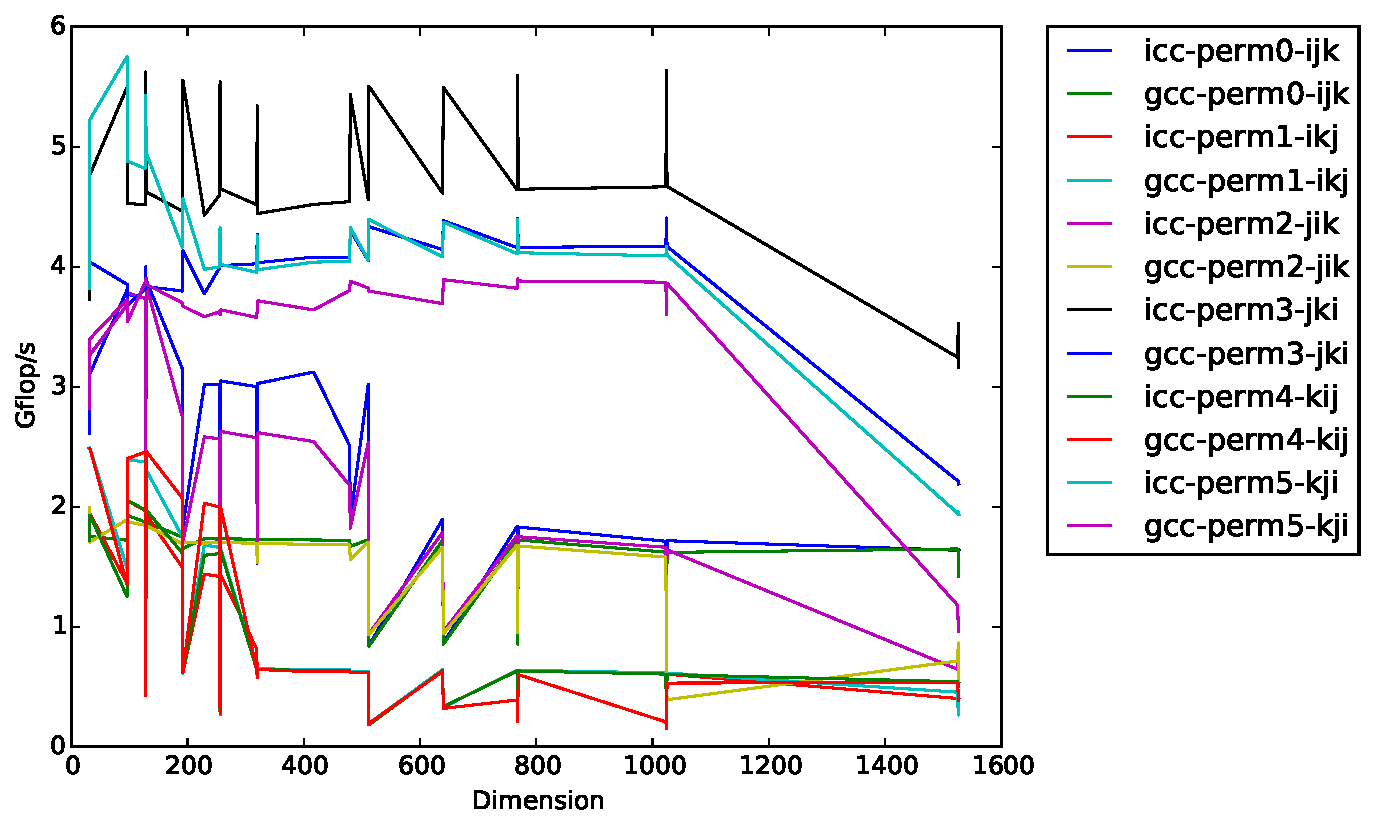
\includegraphics[scale=0.5]{benchmarking/permutations/timing_both.pdf}
\end{center}

\section{Tuning Blocked Matrix Multiply}

Building on previous results, we decided to adopt the optimal \texttt{j-k-i} loop for per-block computation (\texttt{basic\_dgemm}), while searching for an appropriate block size.  We had a two-pronged approach here, which was to

\begin{enumerate}
    \item Guess different block sizes and effectively perform a manual binary search:

    The results of this search, which will be graphed below, indicate that \emph{for the cluster} it seems to be the case that \texttt{BLOCK\_SIZE = 1024} is optimal.

    The testing for this has been done in the file \texttt{dgemm\_blocked\_perm.c}.

    \item Try to programatically find the optimal size.

    This approach has hit somewhat of a dead-end, in that it cannot beat the manual guessing strategy tried first.  The basic idea here is that we have 2 whole matrix blocks that need to fit into memory (\texttt{C} and \texttt{A}), and at each execution of the first nested loop (\texttt{k}) need only grab one element from \texttt{B}.  We made the likely silly assumption that this would mean reading an entire page from memory, so in order to find the ideal \texttt{BLOCK\_SIZE} we need to solve

    $$
    \sqrt{\frac{\text{\ttfamily L3\_SIZE}}{24}} = \text{\ttfamily BLOCK\_SIZE}
    $$

    In code, we have probably made a mistake or fallacious assumption somewhere, or maybe even are just calling the wrong methods with the wrong parameters.  The plotted result below was with a \texttt{BLOCK\_SIZE = 991}, where we hardcoded in 15MB L3 cache to the equation above.  Perhaps this is somewhat reasonable, in the sense that it might make the most sense to take the result of the equation above and round up to the nearest highest power of 2 (which is 1024) since we are working with the cache.

    \noindent The code that was originally purposed for this was in \texttt{dgemm\_basic-permutations.c}.  However, inside of the top of the method \texttt{square\_dgemm} at the bottom of the file you can see the corresponding \texttt{sysconf} calls that are attempting to acquire the right information.  It seems that the calculation we seek to compute for number of per-matrix-block bytes is invalid.  We tried computing having 2 full blocks plus one page (4096 bytes on the cluster), but that produces equally disatisfying results.  The computation in that code is assuming that we need to fit all three matrix blocks in cache at the same time, which is likely not the case.
\end{enumerate}

\noindent The corresponding plot:
\begin{center}
    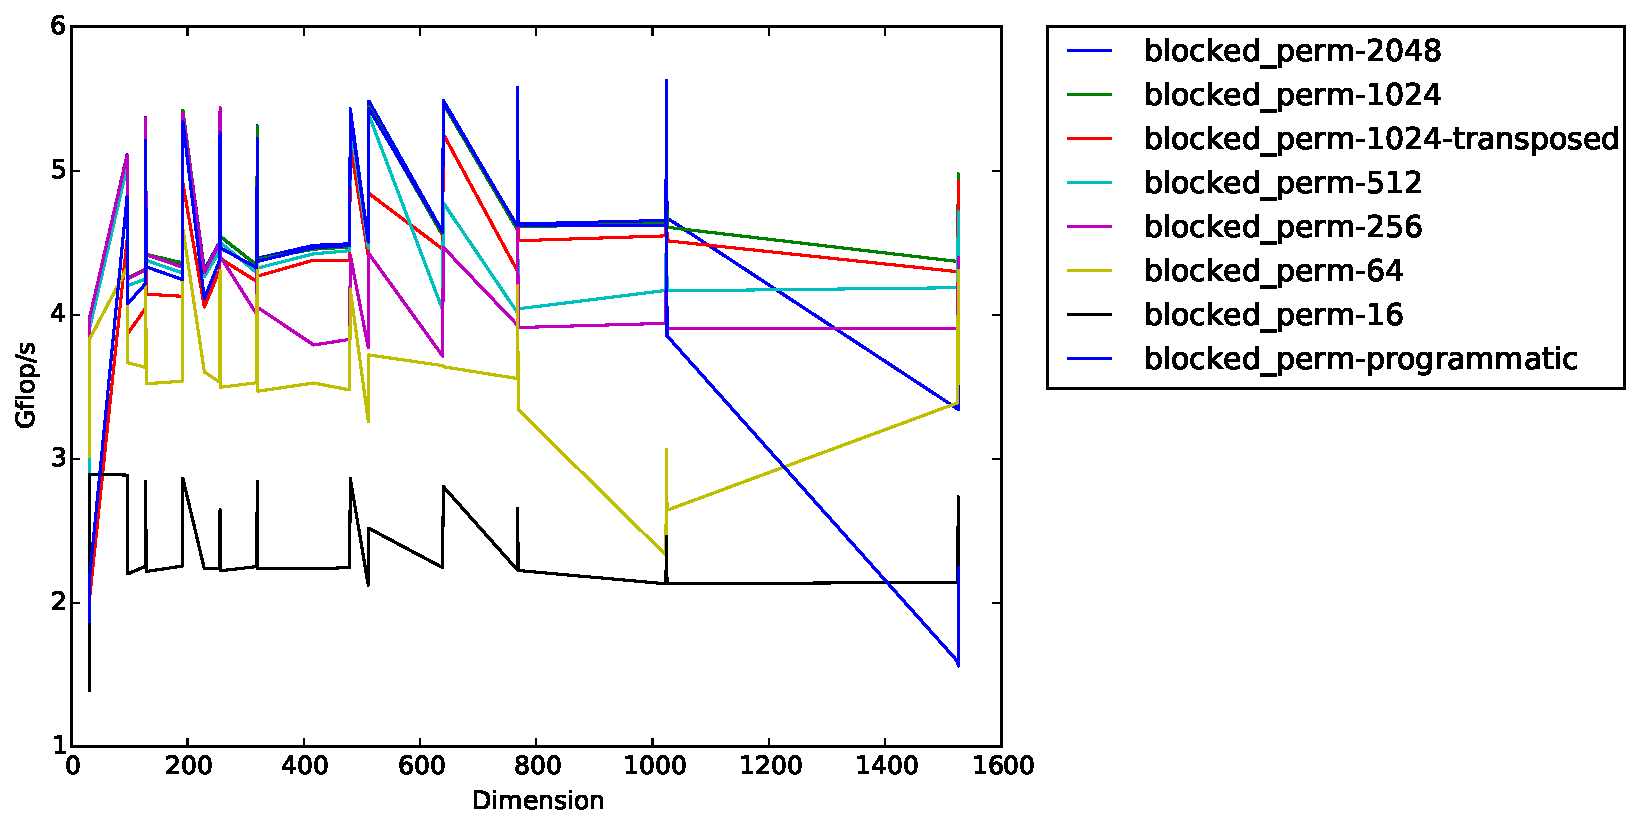
\includegraphics[scale=0.5]{benchmarking/blocked/timing.pdf}
\end{center}

\noindent The plot coloring reset at the bottom for \texttt{blocked\_perm-programmatic}, this is the blue line that degrades \emph{much} faster after a matrix dimension of 1024, for clarity.

\section{Next Stages}

\noindent As a final comparison of some of the methods described above, you can see from the benchmarks that our algorithm is really nothing to be proud of at this point:

\begin{center}
    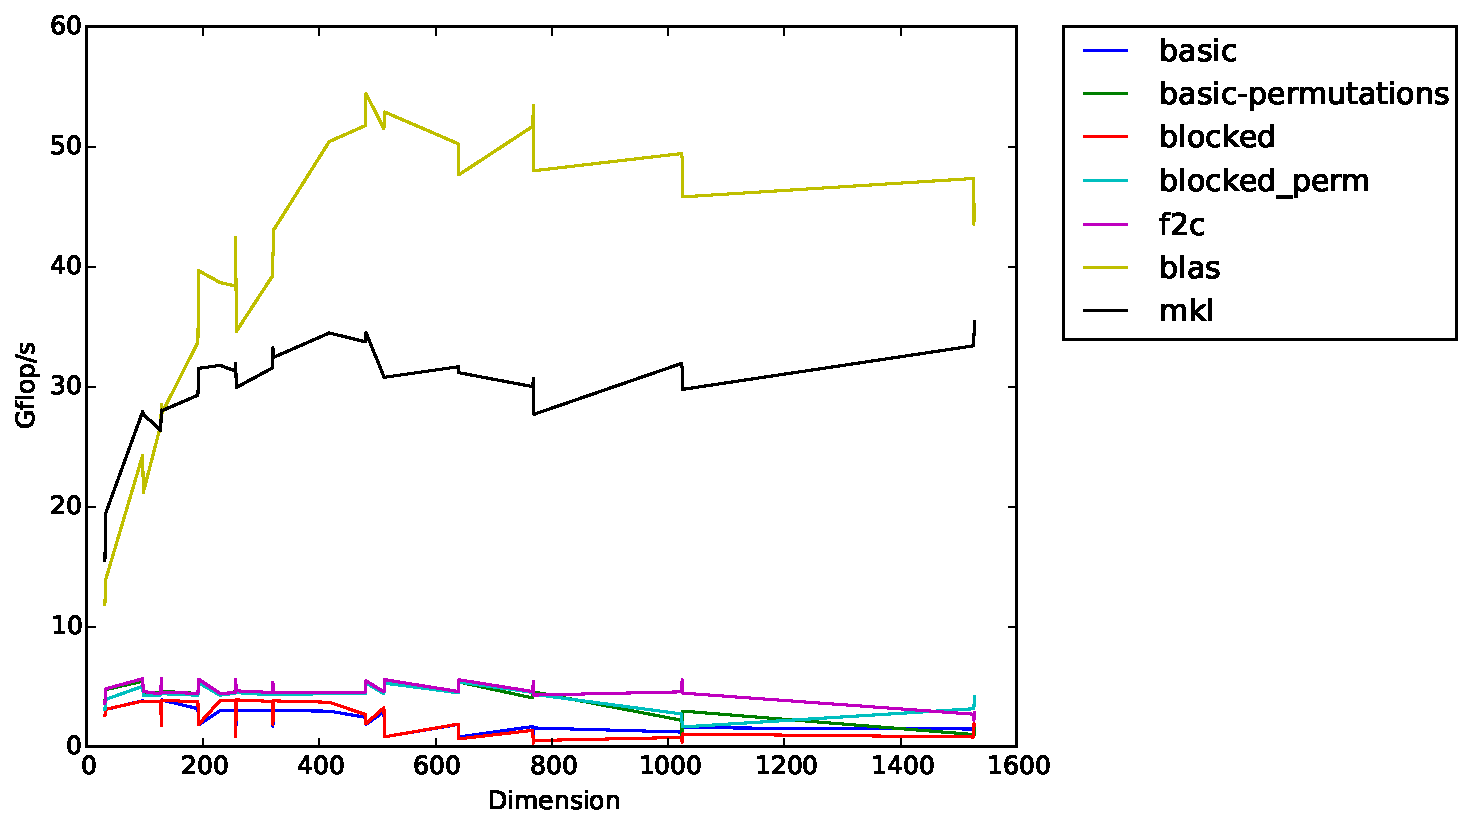
\includegraphics[scale=0.5]{benchmarking/comparison/timing.pdf}
\end{center}

\noindent We have been playing around with transposing things in memory, but generally think that we are not supposed to venture here -- in order to perform such a task with the provided parameters we have to do something like:

\begin{lstlisting}
    double* bad_idea = (double *)(&(*A));
    naive_transpose(M, bad_idea);
\end{lstlisting}

\noindent We also found that the transposed results (also located in \texttt{dgemm\_blocked-ours.c}) really only start having an effect on large matrices since we are looking at an $O(n^2)$ operation in the naive case in order to transpose $A$, and then have to transpose it back.  Asymptotically speaking, as the matrix multiply is $O(n^3)$ we will begin to see better results.\\

\noindent We plan to try new methods such as better copy optimization, compliler flags and annotations, and also want to explore the cache-oblivious variants of this project if possible.

\end{document}
